\graphicspath{{chapters/02/images}}
\chapter{Stochastic Chemical Kinetics}

\section{Rewriting biochemical reactions}
Biochemical reactions are the building blocks to model biological systems.
They provide a unifying notation with sufficient level of details to represent complex biological processes.
Biochemical reactions decorated with reaction kinetics can be simulated by a simulation algorithm to generate a realization of their dynamics.
Chemical species in a biological system move around and gain kinetic energy.
Upon collisions with other species, they undergo reactions to modify and transform into different species.
In order to make this concrete, consider the transformation of a molecule of species A to a molecule of species B.
It is written schematically as $A \rightarrow B$.
This reaction converts one A molecule on the left side of the arrow to a B molecule on the right side.
Such a transforming reaction is called a \emph{unimolecular reaction}.
We are dealing with a structure of compartments, in which we have symbols representing chemicals and \emph{rewriting rules} specifying the direction.
Membrane example: AABC A→B , A→C All these computational systems are more oriented on representation, while if we are more interested in the function we can apply \textbf{equation-based methods}, for instance ODE systems.
In ODE we specify the derivative in time of any of the variables in terms of a function of the state.
The stochastic simulation approach can be approximated by a deterministic one.
The main steps to follow for writing a formal mathematical description of a biological system are\textbf{:}

\begin{enumerate}
  \def\labelenumi{\arabic{enumi}.}
  \item Choose representation: arrow notation
  \item State of the system: integer
  \item Specify the likelihood of execution for each reaction
\end{enumerate}

A reaction will be faster when we have a huge amount of reactants.
Why do we state so? If we think in terms of probability, an example reaction A + B → C will be faster when a there is a high quantity of A and B are present, since it is more likely for them to interact.
Such statement is based on the assumption that there are no gradients in the system, i.e. ~well-mixed chemical system, therefore the distribution of the molecules is uniform.
\textbf{Well-mixed reaction volume}: reaction volume in which all the molecular species are homogeneously distributed and spatially indistinguishable.
Chemical species under the well-mixed assumption at a thermal equilibrium are uniformly distributed in the volume V and their velocities are thermally randomized according to the Maxwell-Boltzmann distribution.
In order to approximate a complex system, we can partition the main compartment in smaller sets where we can apply this assumption - \emph{discretization} procedure.
In terms of stochastic representation we require integers e.g. ~probability that two molecules will interact.
Therefore, Petri nets are a suitable representation for this kind of systems.
\textbf{Formal representation:} The state of a spatially homogeneous biological system is determined by the population of each species, while the position and velocity of each individual molecule are ignored.
Let $X_i(t)$ be the population of species $S_i$ at a particular time t.
The N- vector $X(t) = (X_1(t),...,X_N(t))$, which determines the population of each species, constitutes the system state at the time t.
A general reaction Rj has a general scheme: $v^-_{j1}S_1+...+v^-_{jN}S_N \rightarrow v^+_{j1}S_1+...+v^-_{jN}S_N$ In which a species on the left side of the arrow is called a \emph{reactant}, while a species on the right side is called a \emph{product}.
The non-negative integers $v^-_{ji}$ and $v^+_{ji}$ are the stoichiometric coefficients which denote the number of molecules of a reactant that are consumed and the number of molecules of a product that are produced.
For each reaction $R_j,$ the net change in the population of species $S_i$ involved in the reaction is equal to ($v^+_{ji}- v^-_{ji}$), which can be positive, negative or zero.
The net changes by all reactions are described by a stoichiometry matrix $\mathbf{v}$ with size $M × N$.
The \emph{j}th row $\mathbf{v}_j$ of the stoichiometry matrix expresses the changes caused by reaction $R_j$ and it is called the state change vector.
We can have multiple systems leading to the same stoichiometric matrix.
\textbf{Stoichiometric matrix:}
We require two matrices: $V^+$ provides the products, $V^-$ provides the reactants.

$$ V^- = \begin{bmatrix}1 & 1 & 0 \\ 0 & 1&1 \\ 1&0&1 \end{bmatrix}, V^+ = \begin{bmatrix}0 & 2 & 0 \\ 0 & 0&2 \\ 2&0&0 \end{bmatrix}, V = \begin{bmatrix}1 & 1 & 0 \\ 0 & -1&1 \\ 1&0&-1 \end{bmatrix}\\ V = V^+ + V^- $$

Suppose that at a time t the state (number of molecules in that given moment) is $X(t)$.
it further assumes that the next reaction scheduled to fire at the next time $t + \tau$ is $R _\mu$, which moves the system accordingly to a new state $X(t + \tau)$.
$\mathbf{x}$ is a simple notation to represent $X(t)$.

$$ X(t+\tau) = X(t)+v_\mu $$

\textbf{Summary:} If we want to specify in computational terms the biological system that we are interested into, we end up with the structure of at least one compartment where we assume to have a chemical volume in which there are some entities that interact with each other.
We impose a preliminary assumption, the well-mixed volume, that means that all these actors are available with equal availability in all the parts of the volume.
For each compartment, we need to specify the entities (and how many molecules are available), and the reactions that provide the rules for transforming the chemicals in others along the time.
All these structures of reactions can be defined in mathematical terms using matrices: the number of columns is equal to the number of variables; the number of rows is equal to the number of reactions; the stoichiometric coefficient of reactant or products.

\section{Reaction propensity}
Each reaction in the stochastic chemical kinetics is considered as a stochastic process where each of its occurrences is a random event with an assigned probability distribution.
It is impossible to predict the progress of reactions deterministically, but only stochastically with a probability.
The propensity of a reaction is a formula that is computed on a state of a system.
It is the way that we will use to hint the probability of execution of the reaction.
The propensity $a_j$ of a reaction $R_j$ is defined such that $a_j(x)dt=$ probability that a reaction $ R_j$ fires in the next infinitesimal time interval {[}\emph{t},\emph{t}+\emph{dt}), given the state \emph{X}(\emph{t}) = \textbf{x}at time \emph{t}.
In a chemical setting, the probability of execution of one reaction will be proportional to the viability of the reactant.
The mass action propensity is the expression of the direct proportionality: multiply the rate of the reaction by the counts of the number of distinct combinations of reactants.
The propensity of a reaction is an intrinsic property of the reaction, is linked to the phenomenon that the reaction is going to represent.
The probability will depend on the propensity of the reaction and the other reactions that are competing for the same reactant.
The propensity is not affected by the products.

$$a_1 (0) = c_1 h_1 (x(0))$$

$$h_2(x(0)) = \begin{pmatrix}100 \\ 1 \end{pmatrix}\begin{pmatrix}50 \\ 1 \end{pmatrix}\begin{pmatrix}30 \\ 0 \end{pmatrix}$$

$$x(0+ \tau) = x(0) + V_1 = \begin{bmatrix}99 &51& 30 \end{bmatrix}$$

$$x(0) = \begin{bmatrix}100 &50& 30 \end{bmatrix}$$

Here we are computing the combination, therefore we will not take into account $a^2$ as in the canonical law of mass action.
\textbf{Reaction propensity for reactions $ R_j$ with mass action kinetics}

\begin{itemize}
  \item Synthesis reaction ($\emptyset$ → products): the number of combinations $ h_j = 1 $ and propensity $ a_j =c_j $
  \item Unimolecular reaction ($ S_i$ → products): the number of combinations \emph{h\_j}= \emph{X\_i}and propensity $ a_j = c_jX_i $.
  \item Bimolecular reaction ($ S_i + S_k$ → products): the number of combinations $ h_j = X_iX_k$ and propensity $ a_j = c_jX_iX_k $.
  \item Dimerization reaction ($2S_i$ → products): the number of combinations $ h_j = \frac{1}{2}X_i(X_i -1) $ and propensity $ a_j = \frac{1}{2}c_jX_i(X_i -1) $.
  \item Polymerization reaction ($3S_i$ → products): the number of combinations $ h_j = 16X_i(X_i -1)(X_i -2)$ and propensity $ a_j = 16c_jX_i(X_i -1)(X_i -2) $.
  \item Termolecular reaction ($2S_i + S_k$ → products): the number of combinations $ h_j = \frac{1}{2}X_i(X_i -1)X_k$ and propensity $ a_j = \frac{1}{2}c_jX_i(X_i -1)X_k $.
\end{itemize}

For simulating we need a specification of stoichiometric matrix, a vector of integers (initial values) and stochastic rate.
We will arrive to a formula with which we can compute the probability.
The reaction probability function is required for defining probability.

\section{Chemical Master Equation}
The CME is the theoretical approach allowing to derive the complete set of probability of all possible states of the system.

  \subsection{Grand probability function}
  $\mathbb{P}\{\mathbf{x},t|\mathbf{x}_0,t_o\}$ = probability that the system state is $X(t) = \mathbf{x}$ at time \emph{t}, given the initial state $X(t_0) = \mathbf{x}_0$ at time \emph{t}0.
  By applying the chemical master equation, we end up with a set of differential equations for this probability, which theoretically provide the complete set of any of the state of the system.

  \subsection{CME}

  $$\frac{\mathbb{P}\{\mathbf{x},t|\mathbf{x}_0,t_o\}}{dt}= \sum_{j=1}^{M}(a_j(\mathbf{x}-\mathbf{v}_j)\mathbb{P}\{\mathbf{x},t|\mathbf{x}_0,t_o\})- \mathbb{P}\{\mathbf{x},t|\mathbf{x}_0,t_o\}\sum^M_{j=1}a_j(\mathbf{x})$$

  However, for computing all these probabilities in a complex system, the number of equations will increase and be practically useless.
  The idea is to avoid deriving everything with the chemical master equation but trying to apply another approach that is the one provided by the stochastic simulation.

\section{Stochastic simulation}
When you apply CME you explore all the possible state of the system, with SS you compute only one possible trajectory of the system (for any possibility you must run several time SS, too complex again).
The stochastic simulation works because you only need an idea of the most probable conditions of the system.
SS is faster than a real experiment and you can run it with a computer (you can also run thousands of simulations).

  \subsection{Probability density function}
  The mathematical basis of stochastic simulation is the reaction probability density function (pdf).
  $p(\tau, \mu |\mathbf{x}, t)d\tau$ = probability that a reaction $R_\mu$ fires in the next infinitesimal time interval $[t+\tau,t+\tau+d\tau)$, given the state $X(t) = \mathbf{x}$ at time \emph{t}.
  These probabilities can be computed by considering the idea of propensity.
  The propensity is a formula on the state of the system (depends on some of the variables that are in the system) that allows to provide a quantitative information that can be used to derive the probabilities.
  The propensity is not a probability: propensity is not in a range from 0 to 1 and it is a property of a reaction while the probability is a property of the system.
  One of the crucial points that we must focus on is a way of being able of sampling from this pdf giving the fact that the computer has few ways of generating something that is stochastic.
  In particular, the easiest way is the random number generator.
  The following pseudocode implements this procedure:

  \begin{figure}
    \centering
    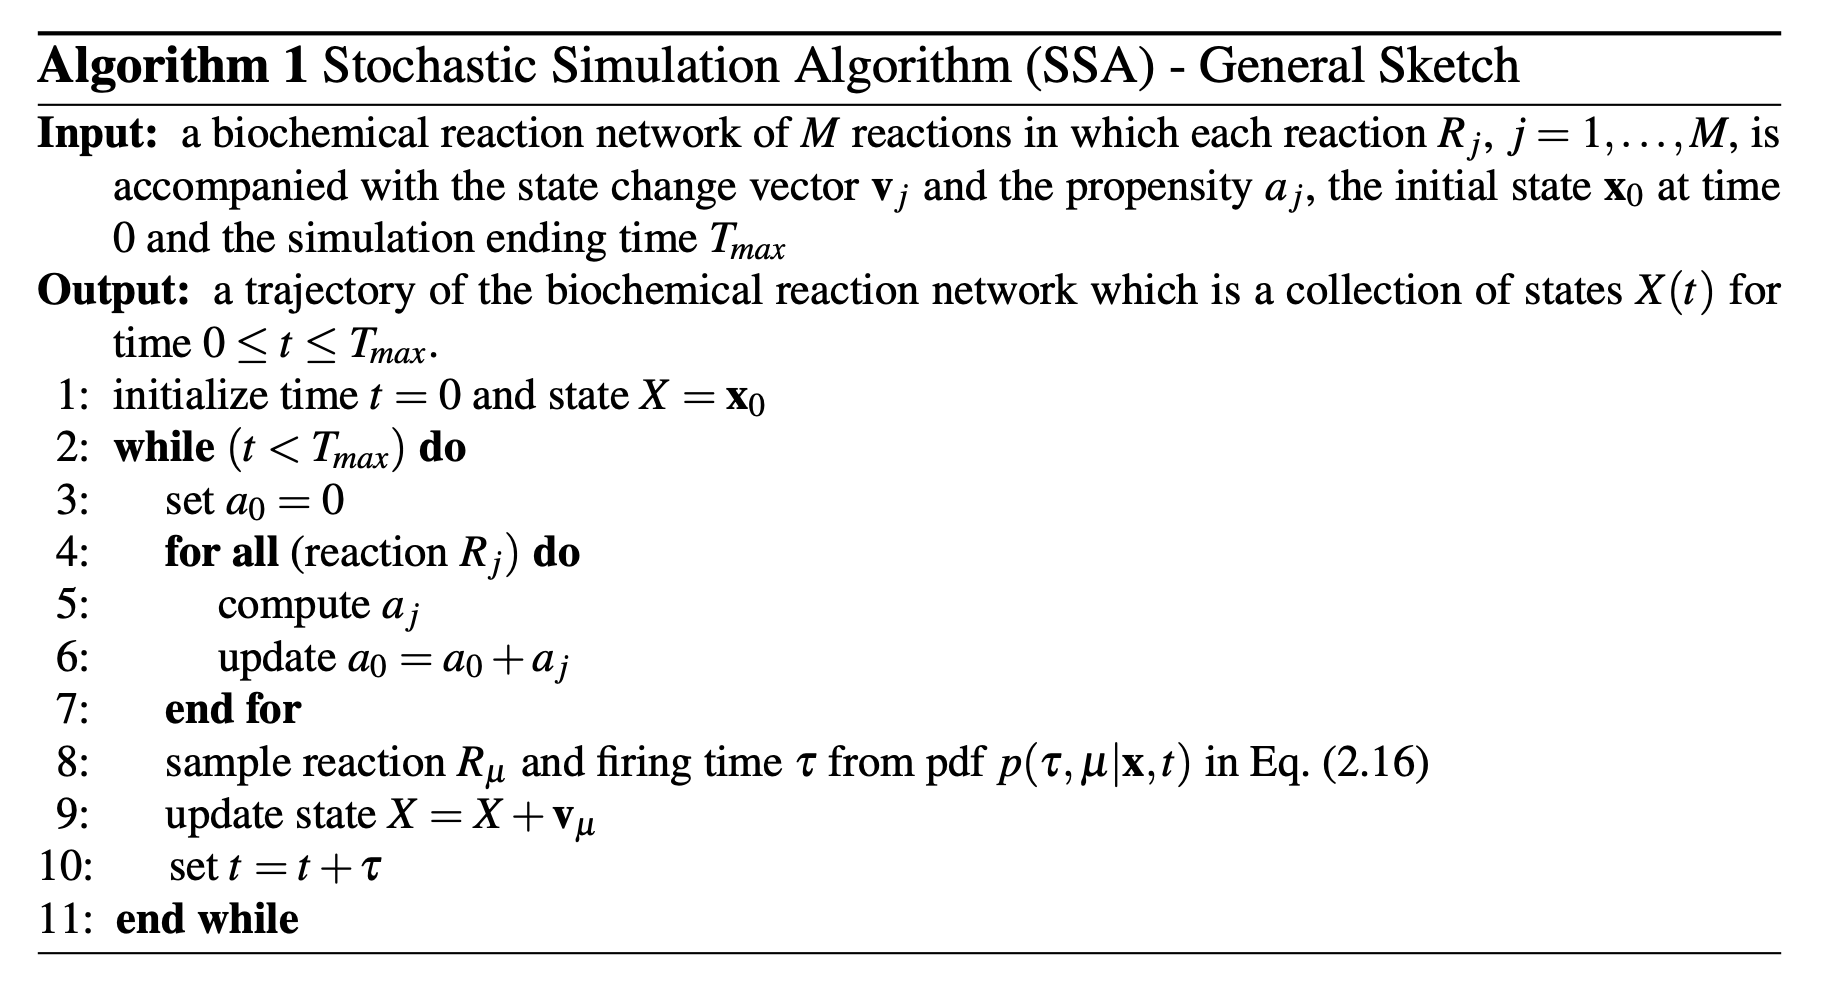
\includegraphics[width=0.7\textwidth]{SSA_algo.png}
    \caption{SSA}
  \end{figure}

  The result of a SSA run is a trajectory, which shows the evolution of the biological system over time.
  The trajectory is a collection of states \emph{X}(\emph{t}) that denotes the state of the system at any time $0 \leq \emph{t}\geq \emph{Tmax}$.
  It should be emphasized that because SSA is a discrete event simulation algorithm, the state changes only at discrete time instants when reactions fire.
  The state between two reaction firings is a constant.
